\documentclass{article} % For LaTeX2e
\usepackage{nips15submit_e,times}
\usepackage{hyperref}
\usepackage{url}
\usepackage{color}
\usepackage{graphicx}
\usepackage{mathtools}


%\documentstyle[nips14submit_09,times,art10]{article} % For LaTeX 2.09


\title{CS 594 Project 2 Report: Representation and Regularization Study of Deep and Wide Neural Network for Image Recognition}


\author{
Yanzi Jin \\
\texttt{yjin25z@uic.edu} \\
\And
Yaru Shi \\
\texttt{yshi31@uic.edu} \\
}

% The \author macro works with any number of authors. There are two commands
% used to separate the names and addresses of multiple authors: \And and \AND.
%
% Using \And between authors leaves it to \LaTeX{} to determine where to break
% the lines. Using \AND forces a linebreak at that point. So, if \LaTeX{}
% puts 3 of 4 authors names on the first line, and the last on the second
% line, try using \AND instead of \And before the third author name.

\newcommand{\fix}{\marginpar{FIX}}
\newcommand{\new}{\marginpar{NEW}}

\nipsfinalcopy % Uncomment for camera-ready version

\begin{document}

\maketitle
\section{Abstract}
Deep Residual Networks (resNet) has demonstrated the state-of-art performance on image classification tasks. Through solving the degradation problem with much simpler architecture, resNet has successfully pushed the depth of neural networks won the first to much higher level. However, the superiority of depth in resNet might also be a weakness of itself. Since there is nothing to force the gradient to learn something from each block, training very deep resNet may cause a problem called diminishing feature reuse, which results in low efficiency in resNet training process. Therefore, various techniques have been addressed on solving this issue. Among them, the Wide Residual Networks (WRN) developed a simple strategy by decreasing the depth and increasing the width of residual networks. Results on CIFAR-10, CIFAR-100 and SVHN shows that WRN can beat the resNet through a simple 16-layer-deep WRN. In this project, firstly we compare the performance of resNet and WRN in various dimension; secondly we experiment with deepening and widening factor to see how these parameters will influence the performance of resNet and WRN; lastly we use some dropout schemas in both depth and width to prevent overfitting in network training. Our findings illustrate that WRN reduces the training time by bringing more parameters in the network training.  \textcolor{red}{Need results}

\section{Introduction}

In recent years, the deep convolutional networks (CNN) have achieved a number of improvements in image recognition tasks. Through convolving convolutional filters with the input image, CNN can produce new features vectors for the next layer, in which early layers contain lower level local features such as edges and color contrasts while deeper layers contain more complicated features such as shapes. While good as it is, CNN is also faced with difficulties in stacking more layers in the training process. One problem is called the vanishing/exploding gradients, which causes a neuron deactivate during training. This problem has been addressed through some initialization techniques such as normalization and intermediate normalization layers. \textcolor{red}{Need reference}. The other problem is degradation, in which accuracy degrades rapidly with the increase of depth. This issue has been addressed the resNet framwork proposed by by He, et. al. \cite{he2015deep}. Instead of directly fitting the desired underlying mapping $H(x)$, the resNet let the stacked nonlinear layers fit the residual of $H(x)$, or namely, $F(x): = H(x) - x$; and recast the original mapping through $F(x)+x$. Due to the formulation of $F(x) + x$ through identity mapping in shortcuts, resNet is able to train networks into very deep levels with no degradation problem. This novel framework has won the competition in ImageNet detection, ImageNet localization, COCO detection, and COCO segmentation.\\*

Although the superiority of resNet is obvious, some researchers also concern the diminishing feature reuse brought by the curse of depth \cite{zagoruyko2016wide}. Diminishing feature reuse is a problem arisen in the forward direction when very deep network is trained. As gradient flows through the network, there is no strict on the resNet such that the gradient has to learn something from the current layer, it is possible that the gradient only decrease in a few blocks, or many blocks share very limited decreasing in the gradient learning. This results in the longness of training time in resNet. Motivated by this, Zagoruyko and Komodakis  \cite{zagoruyko2016wide} introduced a new architecture called Wide Residual Networks (WRN). Experiment shows that WRN can outperform resNet through 16-layer-deep network while 2 times faster training. Of course, such improvement needs certain "sacrifice": the number of parameters needed for training WRN increase exponentially as the width of residual network grows. \\*

With above observations, our project is focused on how to choose between width and depth in the residual networks. Specifically, we increase the number of convolution layers between shortcuts and widen the convolution layer in residual networks. Additionally, we would like to experiment with dropout in ResNet blocks to see how different schemas of dropout might influence the generalization of residual network. Inspired by \cite{he2016identity} and \cite{DBLP:journals/corr/HuangSLSW16}, we are going to integrate the stochastic depth dropout in the resNet and propose a stochastic width dropout scheme. The stochastic depth dropout skips some residual block randomly, while our proposed stochastic width dropout will drop some features randomly. \\*

In the next few paragraphs, we first described the data and techniques used in residual network in Section 3; then we presented the evaluation metrics associated with our research in Section 4; finally we concluded the findings we had during the analyses and discussed the challenges when training the networks in Section 5.

\section{Methods}

\subsection{Data}

In this project, we worked on the CIFAR-10 dataset due to the machine limitation. CIFAR-10 \textcolor{red}{Need references} dataset is a collection of 60000 $32\times 32$ color images in 10 classes, with 6000 images in each class. Among them, 50000 are training samples and the remaining 10000 are testing samples. Figure 1 shows some sample images from each class. 
\begin{figure}[h]
\centering
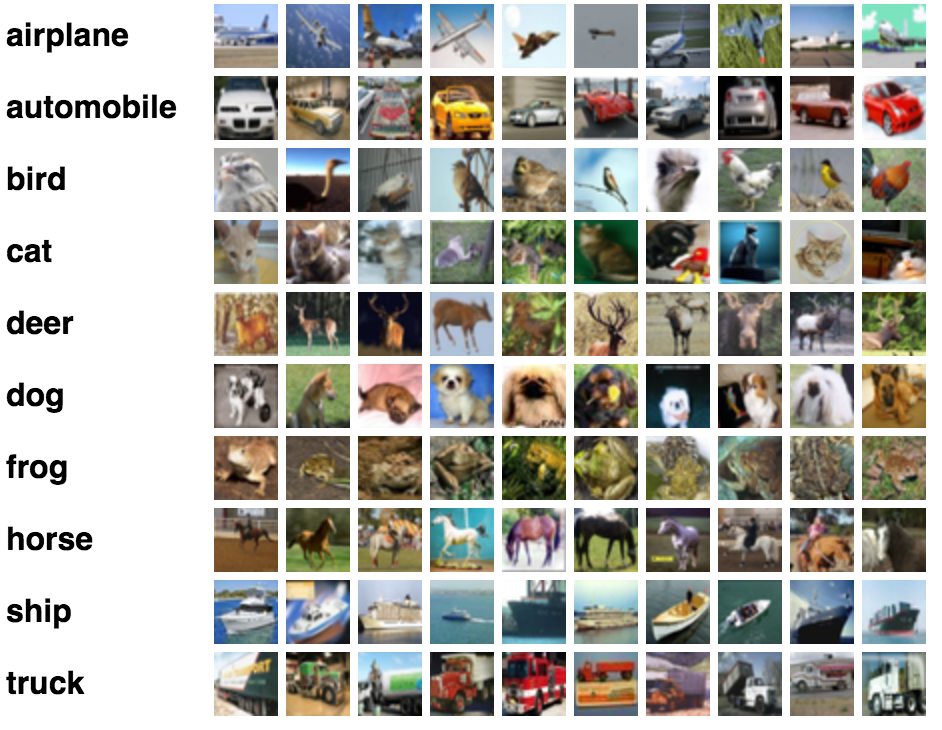
\includegraphics[width=8cm]{cifar10}
 \caption{Sample images for 10 classes from CIFAR-10 dataset}
\end{figure}

\subsection{Deep Residual Network}
Formally, a building block with identity mapping of residual learning is defined as,
\begin{equation}
\boldsymbol{y} = \mathcal{F}(\boldsymbol{x},{W_i}) + \boldsymbol{x}
\end{equation}
Where $\boldsymbol{y}$ and $\boldsymbol{x}$ are the output and input vectors of the current layer.  Function $\mathcal{F}$ is the residual mapping needed to be learned. $W_i$ is the parameter of features in current block.  $\mathcal{F}(\boldsymbol{x},{W_i}) + \boldsymbol{x}$ is an element-wise addition.  This is the reason why it is called identity mapping as $\boldsymbol{x}$ without any changes and it requires the dimensions of $\boldsymbol{x}$ and $\mathcal{F}$ must be equal. Experiments in He et. al. paper showed that identity mapping is simple and effective in solving the degradation problem, therefore no need to add additional projections/parameters for $ \boldsymbol{x}$ unless dimension is unmatched. \\*

Two architectures are used in resNet, a "plain" building block and a "bottleneck" building block. Figure 2 is the simple examples of two block design. The plain block, which is on the left of Figure 2, is the one with two consecutive $3 \times 3$ convolutions with batch normalization and add the identity mapping $\boldsymbol{x}$. The bottleneck block, which is on the right of Figure 2, is consisted of $1 \times 1$, $3 \times 3$, and $1 \times 1$ convolution layers. bottleneck architecture design is crucial in extending the depth of resNet. Experiments showed that resNet with bottleneck was more accurate in prediction and less computationally expensive in layer increasing. Of course, such design of pursuing deeper network is under some sacrifices: each block is very thin and it can only obtain very limited information with small contribution to the final optimization. This is also formulated as a problem called diminishing feature reuse. \\*

\begin{figure}[h]
\centering
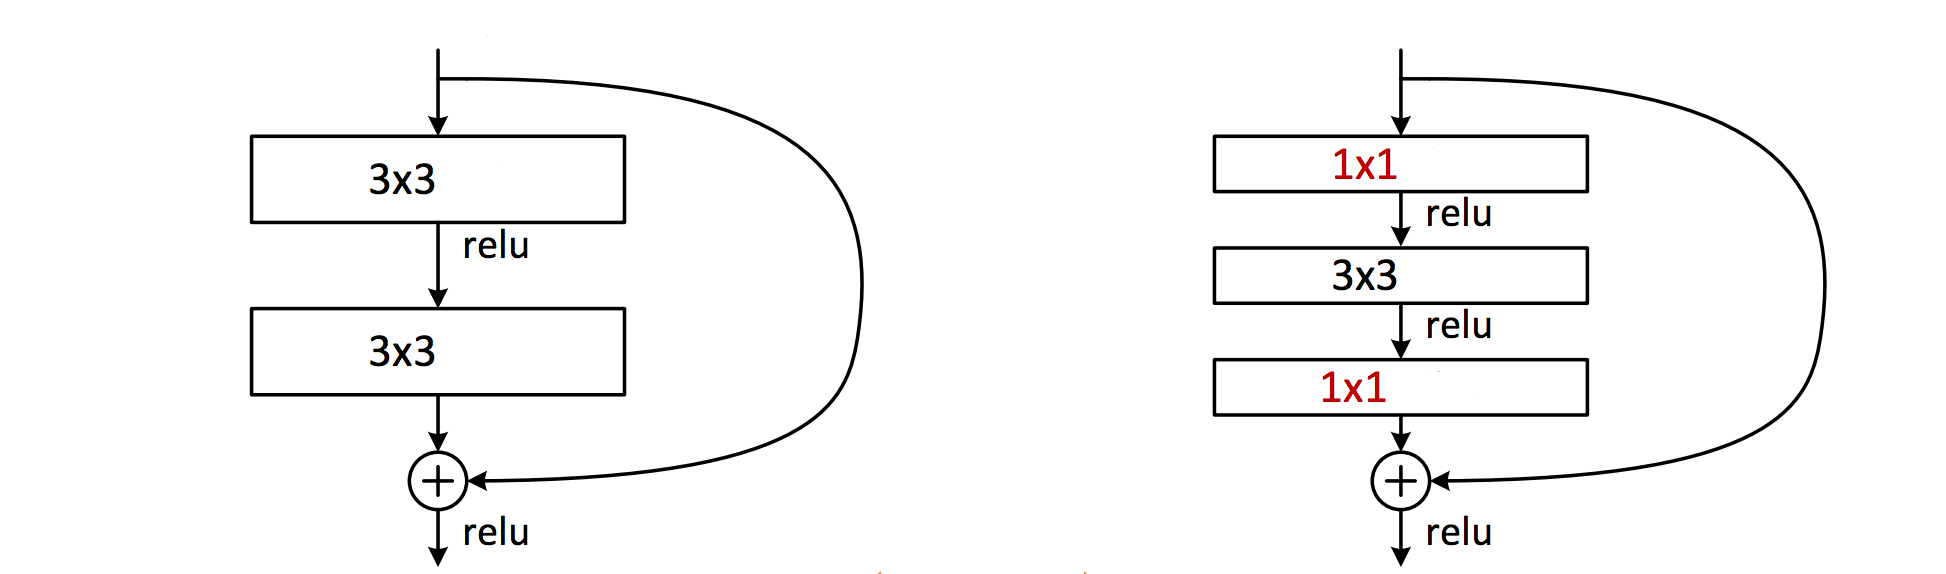
\includegraphics[width=8cm]{bottleneck}
 \caption{Two block structures in resNet}
\end{figure}

\subsection{Wide Residual Network}

Driven by the question that how the width should be address while pursuing depth in resNet, Zagoruyko and Komodakis \cite{zagoruyko2016wide} proposed a novel architecture called Wide Residual Networks (WRN) in 2016. Basically, the idea is to widen the convolutional layers by adding more feature planes. In the paper, they used widen factor k to represent the size of features in convolutional layers compared with baseline block. Figure 3 shows the difference between baseline resNet blocks and WRN blocks, and the baseline block on the left has widen factor $k = 1$ while the wide block on the right has widen factor $k = 2$. Although the computational complexity increases quadraticly with k, WRN is more computational effective on machine due to GPU's superiority in parallel processing in large tensor. Therefore, experiment shows that a 16-layer-deep WRN can have better performance than a regular resNet with much faster computational time. Since the objective of WRN is to widen the resNet, the bottleneck building block was not considered in the paper as its purpose is to make the block thinner. \\*

 \begin{figure}[h]
\centering
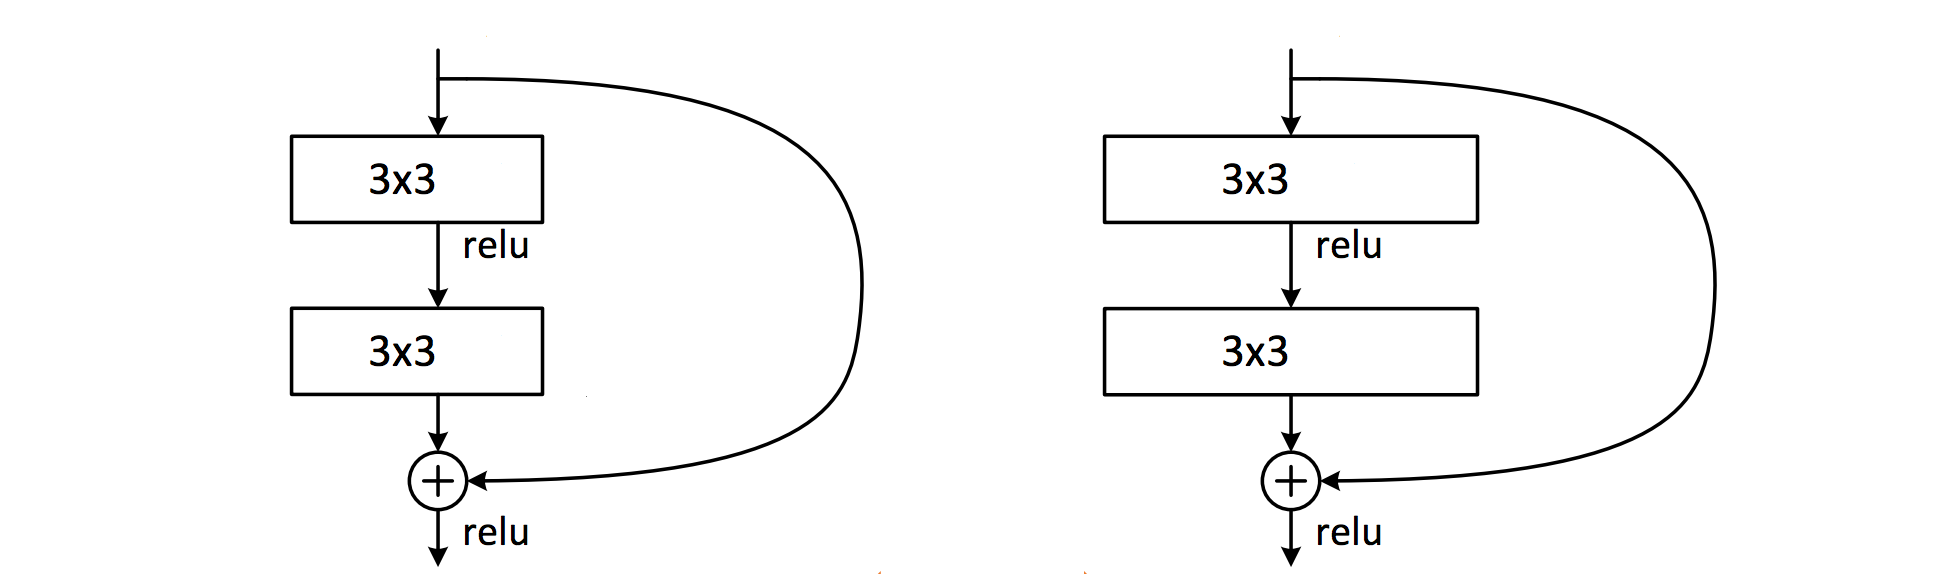
\includegraphics[width=8cm]{wideblock}
 \caption{Narrow block and wide block}
\end{figure}

While Zagoruyko and Komodakis found widen blocks through putting more feature planes can consistently improve the performance of residual network, there are other methods of widening the networks, which might potentially improve the prediction accuracy of residual network. The one we are particularly interested in is to increase the number of layers between dropout per block. Corresponding to the widen factor $k$, this is defined as deepening factor $l$  \cite{zagoruyko2016wide}. Figure 4 shows the comparison between regular building block and the deeper building block. We would like to see if better optimizing the residual in current block will improve the performance of the final network. \\* 

 \begin{figure}[h]
\centering
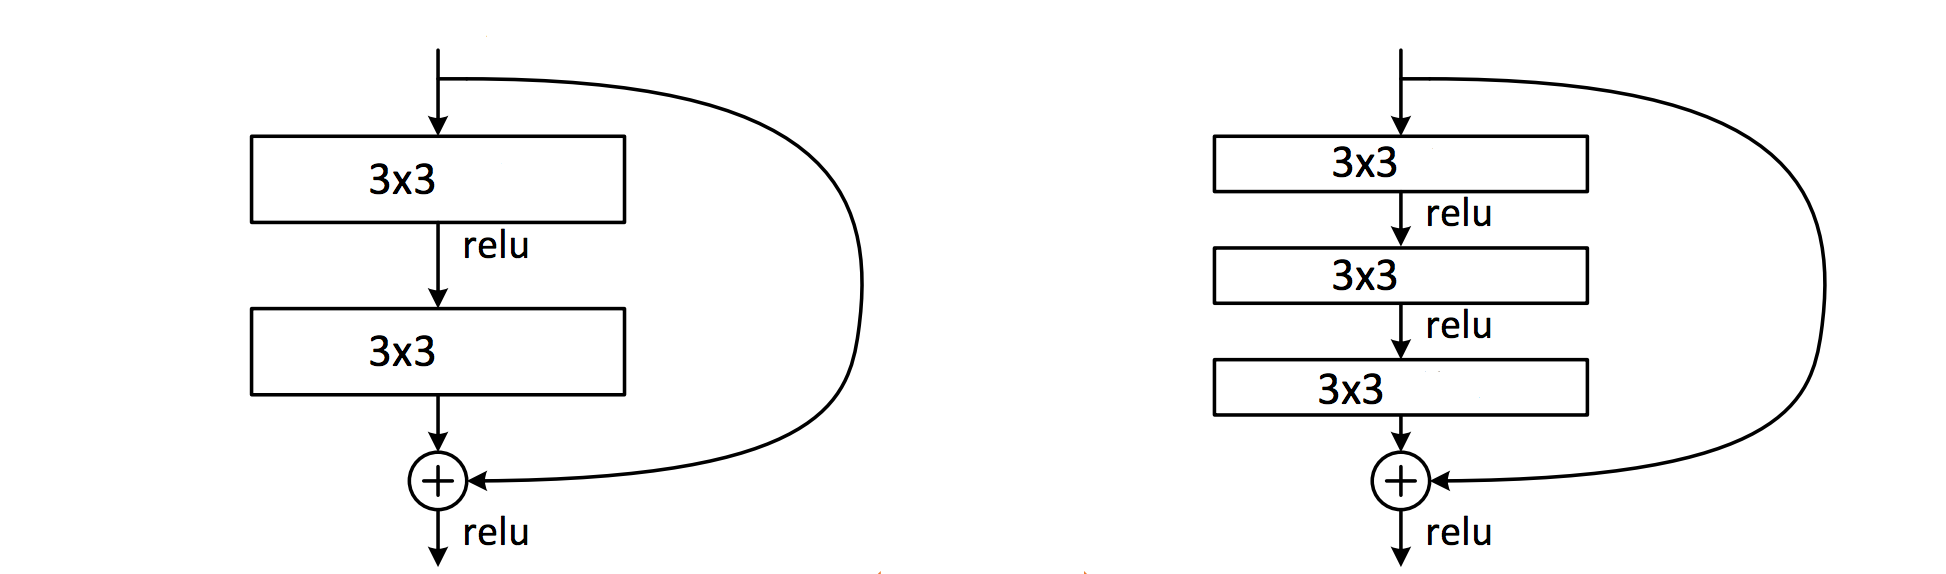
\includegraphics[width=8cm]{deepenfactor}
 \caption{Shallow block and deep block}
\end{figure}

\subsection{Effects of Dropout}

Dropout is a technique for tackling the overfitting problem in deep networks. Basically, the idea is to randomly drop some unites from the network during the training. Such dropouts can reduce the co-adaption among units, therefore generating more independent features for prediction. \\*

There are several strategies to drop the units. The simplest and most widely-used method is to multiply each element in an activation layer by a Bernoulli random variable. Studies  \cite{zagoruyko2016wide}  have shown that using such dropout between convolutional layers instead of in the identity part of block leads to consistent gain in the resNet performance. Another method, called Stochastic Depth \cite{DBLP:journals/corr/HuangSLSW16}, is aim to shrink the depth of network through dropping the whole building block out during the network training. Results on CIFAR-10, CIFAR-100, and ImageNet data show that this method is useful to train very deep networks effectively and efficiently.  Despite the above methods, we would also like to see what happens if we drop one convolutional layer out during the training. Therefore, we proposed a new method and named it as stochastic width. Namely, within each building block of resNet, we multiply each layer of the convolution by a random Bernoulli variable. We expect all three dropout methods should help the generalization of networks, however, due to the small size of CIFAR-10, we expect the benefit might be trivial. 

\section{Evaluation}
\section{Conclusion}















\bibliographystyle{plain}
\bibliography{report} 

\end{document}
